%% abtex2-modelo-trabalho-academico.tex, v-1.9 laurocesar
%% Copyright 2012-2013 by abnTeX2 group at http://abntex2.googlecode.com/ 
%%
%% This work may be distributed and/or modified under the
%% conditions of the LaTeX Project Public License, either version 1.3
%% of this license or (at your option) any later version.
%% The latest version of this license is in
%%   http://www.latex-project.org/lppl.txt
%% and version 1.3 or later is part of all distributions of LaTeX
%% version 2005/12/01 or later.
%%
%% This work has the LPPL maintenance status `maintained'.
%% 
%% The Current Maintainer of this work is the abnTeX2 team, led
%% by Lauro César Araujo. Further information are available on 
%% http://abntex2.googlecode.com/
%%
%% This work consists of the files abntex2-modelo-trabalho-academico.tex,
%% abntex2-modelo-include-comandos and abntex2-modelo-references.bib
%%

% ------------------------------------------------------------------------
% ------------------------------------------------------------------------
% abnTeX2: Modelo de Trabalho Academico (tese de doutorado, dissertacao de
% mestrado e trabalhos monograficos em geral) em conformidade com 
% ABNT NBR 14724:2011: Informacao e documentacao - Trabalhos academicos -
% Apresentacao
% ------------------------------------------------------------------------
% ------------------------------------------------------------------------

\documentclass[
	% -- opções da classe memoir --
	12pt,				% tamanho da fonte
	openright,			% capítulos começam em pág ímpar (insere página vazia caso preciso)
	oneside,			% para impressão em verso e anverso. Oposto a oneside
	a4paper,			% tamanho do papel. 
	% -- opções da classe abntex2 --
	chapter=TITLE,		% títulos de capítulos convertidos em letras maiúsculas
	section=TITLE,		% títulos de seções convertidos em letras maiúsculas
	%subsection=TITLE,	% títulos de subseções convertidos em letras maiúsculas
	%subsubsection=TITLE,% títulos de subsubseções convertidos em letras maiúsculas
	% -- opções do pacote babel --
	english,			% idioma adicional para hifenização
	%french,				% idioma adicional para hifenização
	%spanish,			% idioma adicional para hifenização
	brazil				% o último idioma é o principal do documento
	]{abntex2}

% ---
% PACOTES
% ---

% ---
% Pacotes fundamentais 
% ---
\usepackage{lmodern}			% Usa a fonte Latin Modern			
\usepackage[T1]{fontenc}		% Selecao de codigos de fonte.
%\usepackage[utf8]{inputenc}		% Codificacao do documento (conversão automática dos acentos)
\usepackage{lastpage}			% Usado pela Ficha catalográfica
\usepackage{indentfirst}		% Indenta o primeiro parágrafo de cada seção.
\usepackage{color}				% Controle das cores
\usepackage{graphicx}			% Inclusão de gráficos
\usepackage{microtype} 			% para melhorias de justificação
% ---

\usepackage{listings}
\usepackage{booktabs} %Melhora o visual das tabelas
\usepackage{tabulary} %
\usepackage[table]{xcolor} %
		
% ---
% Pacotes adicionais, usados apenas no âmbito do Modelo Canônico do abnteX2
% ---
\usepackage{lipsum}				% para geração de dummy text
% ---

% ---
% Pacotes de citações
% ---
\usepackage[brazilian,hyperpageref]{backref}	 % Paginas com as citações na bibl
\usepackage[alf]{abntex2cite}	% Citações padrão ABNT

\usepackage{tikz}
\usetikzlibrary{calc,trees,positioning,arrows,chains,shapes.geometric,%
    decorations.pathreplacing,decorations.pathmorphing,shapes,%
    matrix,shapes.symbols}

\tikzset{
	>=stealth',
  punktchain/.style={
    rectangle, 
    rounded corners, 
    % fill=black!10,
    draw=black, very thick,
    text width=10em, 
    minimum height=3em, 
    text centered, 
    on chain},
  line/.style={draw, thick, <-},
  element/.style={
    tape,
    top color=white,
    bottom color=blue!50!black!60!,
    minimum width=8em,
    draw=blue!40!black!90, very thick,
    text width=10em, 
    minimum height=3.5em, 
    text centered, 
    on chain},
  every join/.style={->, thick,shorten >=1pt},
  decoration={brace},
  tuborg/.style={decorate},
  tubnode/.style={midway, right=2pt},
}

% --- 
% CONFIGURAÇÕES DE PACOTES
% --- 

% ---
% Configurações do pacote backref
% Usado sem a opção hyperpageref de backref
\renewcommand{\backrefpagesname}{Citado na(s) página(s):~}
% Texto padrão antes do número das páginas
\renewcommand{\backref}{}
% Define os textos da citação
\renewcommand*{\backrefalt}[4]{
	\ifcase #1 %
		Nenhuma citação no texto.%
	\or
		Citado na página #2.%
	\else
		Citado #1 vezes nas páginas #2.%
	\fi}%
% ---

% ---
% Informações de dados para CAPA e FOLHA DE ROSTO
% ---
\titulo{\textsc{Modelo de Banco de Dados para Gerenciamento de Pizzaria: Modelagem e Implementação}}
\autor{Guilherme Augusto de Macedo \and Matheus Liberato Domingues da Silva \and Victor Hugo Carlquist da Silva}
\local{Campos do Jordão}
\data{2013}
\orientador{Paulo Giovani de Faria Zeferino}
% \coorientador{Equipe \abnTeX}
\instituicao{Instituto Federal de Educação, Ciência e Tecnologia de São Paulo - \textit{campus} Campos do Jordão}
\tipotrabalho{Trabalho Final}
% O preambulo deve conter o tipo do trabalho, o objetivo, 
% o nome da instituição e a área de concentração 
\preambulo{Trabalho final apresentado na disciplina de Banco de Dados II no quarto módulo do curso de Tecnologia em Análise e Desenvolvimento de Sistemas do IFSP-CJO.}


% Configurações de aparência do PDF final

% alterando o aspecto da cor azul
\definecolor{blue}{RGB}{41,5,195}

% informações do PDF
\makeatletter
\hypersetup{
     	%pagebackref=true,
		pdftitle={\@title}, 
		pdfauthor={\@author},
    	pdfsubject={\imprimirpreambulo},
	    pdfcreator={LaTeX with abnTeX2},
		pdfkeywords={abnt}{latex}{abntex}{abntex2}{trabalho acadêmico}, 
		colorlinks=true,       		% false: boxed links; true: colored links
    	linkcolor=blue,          	% color of internal links
    	citecolor=blue,        		% color of links to bibliography
    	filecolor=magenta,      	% color of file links
		urlcolor=blue,
		bookmarksdepth=4
}
\makeatother
% --- 

% --- 
% Espaçamentos entre linhas e parágrafos 
% --- 

% O tamanho do parágrafo é dado por:
\setlength{\parindent}{1.3cm}

% Controle do espaçamento entre um parágrafo e outro:
\setlength{\parskip}{0.2cm}  % tente também \onelineskip

% ---
% compila o indice
% ---
\makeindex
% ---

\lstset{language=SQL,
	basicstyle = \ttfamily\footnotesize, % Tamanho da fonte do código
	numbers = left, % Posição da numeração das linhas
	numberstyle = \tiny\color{blue}, % Estilo da numeração de linhas
	stepnumber = 1, % Numeração das linhas ocorre a cada quantas linhas?
	numbersep = 10pt, % Distância entre a numeração das linhas e o código
	backgroundcolor = \color{white}, % Cor de fundo
	showspaces = false, % Exibe espaços com um sublinhado
	showstringspaces = false, % Sublinha espaços em Strings
	showtabs = false, % Exibe tabulação com um sublinhado
	frame = l, % Envolve o código com uma moldura, pode ser single ou trBL
	rulecolor = \color{black}, % Cor da moldura
	tabsize = 2, % Configura tabulação em x espaços
	captionpos = b, % Posição do título pode ser t (top) ou b (bottom)
	breaklines = true, % Configura quebra de linha automática
	breakatwhitespace= false, % Configura quebra de linha
	%title = \lstname, % Exibe o nome do arquivo incluido
	%caption = \lstname, % Também é possível usar caption no lugar de title
	keywordstyle = \color{blue}, % Estilo das palavras chaves
	commentstyle = \color{green}, % Estilo dos Comentários
	stringstyle = \color{red}, % Estilo de Strings
	escapeinside = {\%*}{*)}, % Permite adicionar comandos LaTeX dentro doseu có digo
	morekeywords ={*,USE,GO} % Se quiser adicionar mais palavras-chave
}

% ----
% Início do documento
% ----
\begin{document}

% Retira espaço extra obsoleto entre as frases.
\frenchspacing 

% ----------------------------------------------------------
% ELEMENTOS PRÉ-TEXTUAIS
% ----------------------------------------------------------
% \pretextual

% ---
% Capa
% ---
\imprimircapa
% ---

% ---
% Folha de rosto
% (o * indica que haverá a ficha bibliográfica)
% ---
\imprimirfolhaderosto*
% ---

% ---
% Inserir a ficha bibliografica
% ---

% Isto é um exemplo de Ficha Catalográfica, ou ``Dados internacionais de
% catalogação-na-publicação''. Você pode utilizar este modelo como referência. 
% Porém, provavelmente a biblioteca da sua universidade lhe fornecerá um PDF
% com a ficha catalográfica definitiva após a defesa do trabalho. Quando estiver
% com o documento, salve-o como PDF no diretório do seu projeto e substitua todo
% o conteúdo de implementação deste arquivo pelo comando abaixo:
%
% \begin{fichacatalografica}
%     \includepdf{fig_ficha_catalografica.pdf}
% \end{fichacatalografica}
\begin{fichacatalografica}
	\vspace*{\fill}					% Posição vertical
	\hrule							% Linha horizontal
	\begin{center}					% Minipage Centralizado
	\begin{minipage}[c]{12.5cm}		% Largura
	
	\imprimirautor
	
	\hspace{0.5cm} \imprimirtitulo  / \imprimirautor. --
	\imprimirlocal, \imprimirdata-
	
	\hspace{0.5cm} \pageref{LastPage} p. : il. (algumas color.) ; 30 cm.\\
	
	\hspace{0.5cm} \imprimirorientadorRotulo~\imprimirorientador\\
	
	\hspace{0.5cm}
	\parbox[t]{\textwidth}{\imprimirtipotrabalho~--~\imprimirinstituicao,
	\imprimirdata.}\\
	
	\hspace{0.5cm}
		1. Complexidade de Algoritmo.
		2. Processamento de Imagens.
		I. Autor.
		II. Título
		III. Orientador.
		IV. Faculdade.
		V. Título\\ 			
	
	\hspace{8.75cm} CDU 02:141:005.7\\
	
	\end{minipage}
	\end{center}
	\hrule
\end{fichacatalografica}
% ---


% ---
% Inserir folha de aprovação
% ---

% Isto é um exemplo de Folha de aprovação, elemento obrigatório da NBR
% 14724/2011 (seção 4.2.1.3). Você pode utilizar este modelo até a aprovação
% do trabalho. Após isso, substitua todo o conteúdo deste arquivo por uma
% imagem da página assinada pela banca com o comando abaixo:
%
% \includepdf{folhadeaprovacao_final.pdf}
%
\begin{folhadeaprovacao}

  \begin{center}
    {\ABNTEXchapterfont\large\imprimirautor}

    \vspace*{\fill}\vspace*{\fill}
    \begin{center}
      \ABNTEXchapterfont\bfseries\Large\imprimirtitulo
    \end{center}
    \vspace*{\fill}
    
    \hspace{.45\textwidth}
    \begin{minipage}{.5\textwidth}
        \imprimirpreambulo
    \end{minipage}%
    \vspace*{\fill}
   \end{center}
        
   % Trabalho aprovado. \imprimirlocal, 29 de outubro de 2013:
   \begin{center}
   	\noindent\textbf{\large Banca Examinadora}\\
   	\noindent 03 de dezembro de 2013
   \end{center}

   \assinatura{\textbf{Prof. \imprimirorientador} \\ Orientador} 
   \assinatura{\textbf{Prof. Me. Alvaro Costa Neto} \\ Convidado 1}
   \assinatura{\textbf{Prof. Esp. Alisson Ribeiro} \\ Convidado 2}
   %\assinatura{\textbf{Professor} \\ Convidado 3}
   %\assinatura{\textbf{Professor} \\ Convidado 4}
      
   \begin{center}
    \vspace*{0.5cm}
    {\large\imprimirlocal}
    \par
    {\large\imprimirdata}
    \vspace*{1cm}
  \end{center}
  
\end{folhadeaprovacao}
% ---

% ----------------------------------------------------------
% RESUMOS
% ----------------------------------------------------------

% resumo em português
\setlength{\absparsep}{18pt} % ajusta o espaçamento dos parágrafos do resumo
\begin{resumo}
	Lorem ipsum dolor sit amet, consectetur adipisicing elit, sed do eiusmod
	tempor incididunt ut labore et dolore magna aliqua. Ut enim ad minim veniam,
	quis nostrud exercitation ullamco laboris nisi ut aliquip ex ea commodo
	consequat. Duis aute irure dolor in reprehenderit in voluptate velit esse
	cillum dolore eu fugiat nulla pariatur. Excepteur sint occaecat cupidatat non
	proident, sunt in culpa qui officia deserunt mollit anim id est laborum.Lorem ipsum dolor sit amet, consectetur adipisicing elit, sed do eiusmod
	tempor incididunt ut labore et dolore magna aliqua. Ut enim ad minim veniam,
	quis nostrud exercitation ullamco laboris nisi ut aliquip ex ea commodo
	consequat. Duis aute irure dolor in reprehenderit in voluptate velit esse
	cillum dolore eu fugiat nulla pariatur. Excepteur sint occaecat cupidatat non
	proident, sunt in culpa qui officia deserunt mollit anim id est laborum.Lorem ipsum dolor sit amet, consectetur adipisicing elit, sed do eiusmod
	tempor incididunt ut labore et dolore magna aliqua. Ut enim ad minim veniam,
	quis nostrud exercitation ullamco laboris nisi ut aliquip ex ea commodo
	consequat. Duis aute irure dolor in reprehenderit in voluptate velit esse
	cillum dolore eu fugiat nulla pariatur. Excepteur sint occaecat cupidatat non
	proident, sunt in culpa qui officia deserunt mollit anim id est laborum.

 \textbf{Palavras-chaves}: Complexidade de Algoritmos. Processamento de Imagens. Computação Heterogênea.
\end{resumo}

% resumo em inglês
\begin{resumo}[Abstract]
 \begin{otherlanguage*}{english}
   	Lorem ipsum dolor sit amet, consectetur adipisicing elit, sed do eiusmod
	tempor incididunt ut labore et dolore magna aliqua. Ut enim ad minim veniam,
	quis nostrud exercitation ullamco laboris nisi ut aliquip ex ea commodo
	consequat. Duis aute irure dolor in reprehenderit in voluptate velit esse
	cillum dolore eu fugiat nulla pariatur. Excepteur sint occaecat cupidatat non
	proident, sunt in culpa qui officia deserunt mollit anim id est laborum.Lorem ipsum dolor sit amet, consectetur adipisicing elit, sed do eiusmod
	tempor incididunt ut labore et dolore magna aliqua. Ut enim ad minim veniam,
	quis nostrud exercitation ullamco laboris nisi ut aliquip ex ea commodo
	consequat. Duis aute irure dolor in reprehenderit in voluptate velit esse
	cillum dolore eu fugiat nulla pariatur. Excepteur sint occaecat cupidatat non
	proident, sunt in culpa qui officia deserunt mollit anim id est laborum.Lorem ipsum dolor sit amet, consectetur adipisicing elit, sed do eiusmod
	tempor incididunt ut labore et dolore magna aliqua. Ut enim ad minim veniam,
	quis nostrud exercitation ullamco laboris nisi ut aliquip ex ea commodo
	consequat. Duis aute irure dolor in reprehenderit in voluptate velit esse
	cillum dolore eu fugiat nulla pariatur. Excepteur sint occaecat cupidatat non
	proident, sunt in culpa qui officia deserunt mollit anim id est laborum.
   \vspace{\onelineskip}
 
   \noindent 
   \textbf{Key-words}: Algorithm Complexity. Image Procesing. Heterogeneous Computing.
 \end{otherlanguage*}
\end{resumo}

% ---
% inserir lista de ilustrações
% ---
\pdfbookmark[0]{\listfigurename}{lof}
\listoffigures*
\cleardoublepage
% ---

% ---
% inserir lista de tabelas
% ---
\pdfbookmark[0]{\listtablename}{lot}
\listoftables*
\cleardoublepage
% ---

% ---
% inserir lista de abreviaturas e siglas
% ---
% \begin{siglas}
%   \item[DFA] Detrended Fluctuation Analysis
%   \item[DFA 2D] Two-Dimesional Detrended Fluctuation Analysis
%   \item[GPU] Graphics Processing Unit
%   \item[FPGA] Field-programmable Gate Arrays
%   \item[GPGPU] General Propose GPU
% \end{siglas}
% ---

% ---
% inserir lista de símbolos
% ---
% \begin{simbolos}
%   \item[$ \Gamma $] Letra grega Gama
%   \item[$ \Lambda $] Lambda
%   \item[$ \zeta $] Letra grega minúscula zeta
%   \item[$ \in $] Pertence
% \end{simbolos}
% ---

% ---
% inserir o sumario
% ---
\pdfbookmark[0]{\contentsname}{toc}
\tableofcontents*
\cleardoublepage
% ---

% ----------------------------------------------------------
% ELEMENTOS TEXTUAIS
% ----------------------------------------------------------
\textual

% ----------------------------------------------------------
% Intrudução
% ----------------------------------------------------------
\chapter*[Introdução]{Introdução}
\addcontentsline{toc}{chapter}{Introdução}
    O projeto proposto tem por objetivo a modelagem conceitual, lógica e física de um projeto de Banco de Dados
    para gerenciamento/automatização de uma pizzaria. 

    Depois de gerado o modelo físico, implementou-se a solução utilizando o \textit{SQL Server Management Studio}. 
    Com base nessa implementação, consultas, \textit{views}, \textit{triggers}, entre outras rotinas, foram criadas para 
    fins de execução e testes.
    
    Os capítulos seguintes estão divididos em Metodologia Proposta, onde é detalhada a metodologia utilizada para a 
    execução o projeto, seguidos de explicações a respeito do modelo conceitual, lógico e físico. Posteriormente, 
    as consultas realizadas são explicadas, assim como o restante das rotinas elaboradas.

% ----------------------------------------------------------
% Metodologia Proposta
% ----------------------------------------------------------
\chapter{Metodologia Proposta}

Para a execução dessa trabalho a metodologia foi dividida em três 
etapas: \emph{Criação do modelo conceitual}, \emph{Criação do modelo lógico}, 
\emph{Criação do modelo físico}, \emph{Implementação} e \emph{Execução e Testes}. 
A figura \ref{figuramet} ilustra a sequência de execução destas etapas.

\begin{figure}[h]
    \caption{Epatas da metodologia}
    \centering

    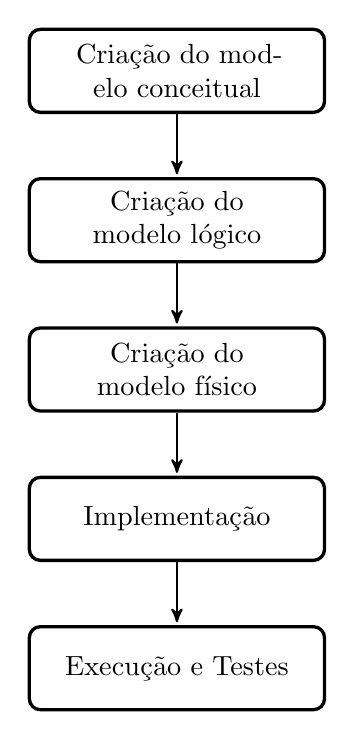
\begin{tikzpicture}
      [node distance=.8cm, start chain=going below,]
         \node[punktchain, join] (etapa1) {Criação do modelo conceitual};
         \node[punktchain, join] (etapa2) {Criação do modelo lógico};
         \node[punktchain, join] (etapa3) {Criação do modelo físico};
         \node[punktchain, join] (etapa4) {Implementação};
         \node[punktchain, join] (etapa5) {Execução e Testes};
    \end{tikzpicture}

    \legend{Fonte: Autor}
    \label{figuramet}
\end{figure}

% ----------------------------------------------------------
% Regras de Negócio
% ----------------------------------------------------------
\chapter {Regras de Negócio}

A modelagem foi realizada tomando por base as seguintes regras de negócio
    requisitos:
    \begin {enumerate}
        \item Opção de realização de pedidos online;
        \item Pizzaria delivery;
        \item Após cadastro, opção do cliente cadastrar dependentes;
        \item Registro de admissão e demissão de funcionários;
        \item Log automático das atividades dos funcionários;
        \item Controle de estoque com base nos fornecedores e nos ingredientes das pizzas;
        \item Esquema de backup automático da base de dados.
    \end {enumerate}

% ----------------------------------------------------------
% Modelo Conceitual
% ----------------------------------------------------------
\chapter{Modelo Conceitual}
    O modelo conceitual foi elaborado no programa \textit{BrModelo}. A Figura \ref{mc01} 
    mostra como foi feita a modelagem para que os pedidos realizados pelos funcionários fossem 
    armazenados na tabela \textit{Log}. Isso é feito através de triggers.
    
    \begin{figure}[h]
         \centering
         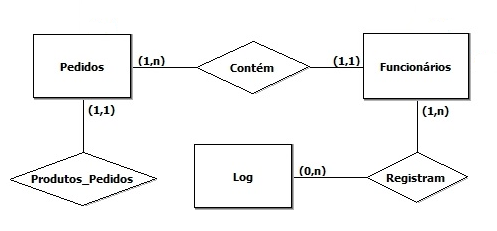
\includegraphics[width=15cm,keepaspectratio]{Imgs/MC_01}
         \caption{Utilização de triggers para alimentar a tabela \textit{Log}}.
         \label{mc01}
    \end{figure}    

    \newpage
    
    Na Figura \ref{mc_02} é possível notar que cada funcionário pode term 
    nenhum ou vários dependentes. Também é possível observar que os clientes podem 
    realizar nenhum ou vários pedidos, mas cada pedido pertence a um único cliente.
    \begin{figure}[h]
         \centering
         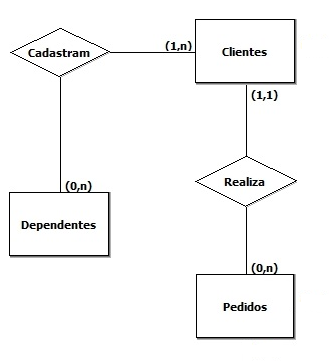
\includegraphics[width=10cm,keepaspectratio]{Imgs/MC_02}
         \caption{Entidades: Dependentes, Clientes e Pedidos.}
         \label{mc_02}
    \end{figure}

    \newpage

    De acordo com a Figura \ref{mc_03}, é possível observar que o 
    Fornecedor alimenta o estoque e os produtos são feitos com ingredientes 
    retirados do estoque.
    \begin{figure}[h]
         \centering
         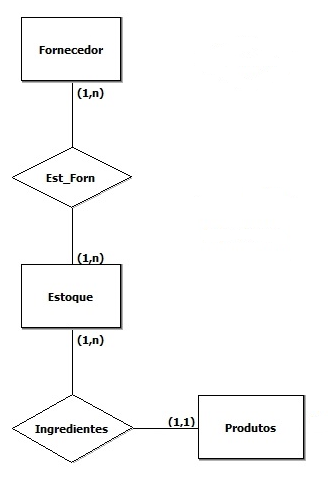
\includegraphics[width=10cm,keepaspectratio]{Imgs/MC_03}
         \caption{Entidades: Fornecedor, Estoque e Produtos}
         \label{mc_03}
    \end{figure}

    \newpage
    
    Na Figura \ref{mc_00} é possível observar como ficou a modelagem completa 
    do sistema.
    \begin{figure}[h]
         \centering
         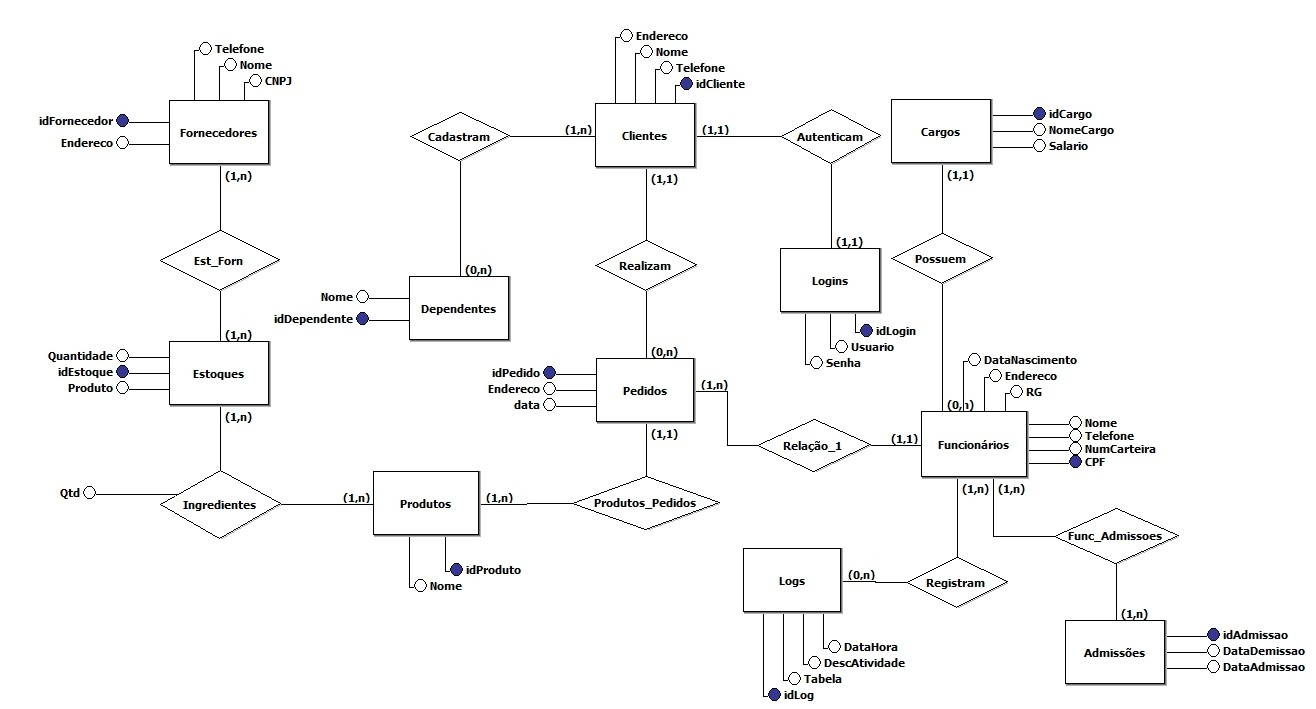
\includegraphics[width=20cm,keepaspectratio,angle=90]{Imgs/MC_00}
         \caption{Modelo Conceitual Completo.}
         \label{mc_00}
    \end{figure}    

% ----------------------------------------------------------
% Modelo Lógico
% ----------------------------------------------------------
\chapter{Modelo Lógico}
    
    A Figura \ref{ml_01} representa, conforme o modelo conceitual, a possibilidade do 
    cliente ter ou não login. Isso não impede que o mesmo efetue pedido. Isso aconteceria, 
    por exemplo, no caso do cliente nunca ter feito pedido online.
    \begin{figure}[h]
         \centering
         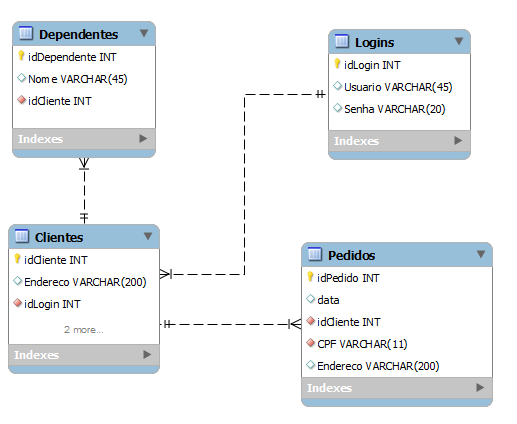
\includegraphics[width=10cm,keepaspectratio]{Imgs/ML_01}
         \caption{Modelo Lógico: Dependentes, Clientes, Logins e Pedidos}
         \label{ml_01}
    \end{figure}
    
    \newpage
    
    Na Figura \ref{ml_02} é possível observar os produtos sendo compostos por um ou mais ingredientes; 
    os ingredientes sendo compostos por um ou mais itens do estoque, mas cada item do estoque podendo 
    ser utilizado apenas em uma lista de ingredientes. Também é possível observar a tabela Estoques\_Fornecedores, 
    podendo conter vários fornecedores vários itens para o estoque.
    \begin{figure}[h]
         \centering
         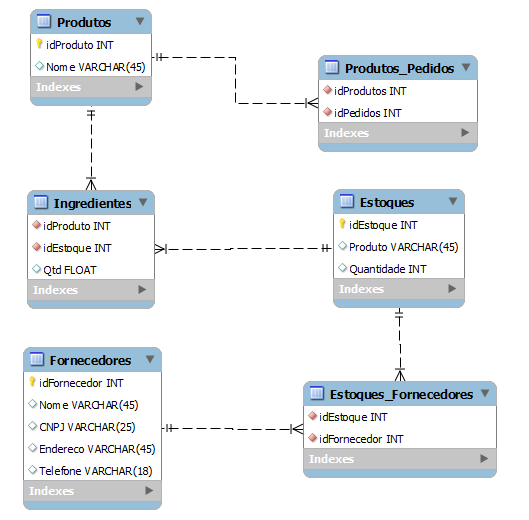
\includegraphics[width=10cm,keepaspectratio]{Imgs/ML_02}
         \caption{Modelo Lógico: Produtos, Ingredientes, Produtos\_Pedidos, Estoques, Estoques\_Fornecedores e Fornecedores.}
         \label{ml_02}
    \end{figure}
    
        \newpage
    
    A Figura \ref{ml_03} mostra a tabela Logs dos funcionários. Essa tabela guarda todas as ações dos 
    funcionários para possível auditorias. É possível observar também que os funcionários têm cargos e 
    cada cargo pode ter muitos funcionários, mas cada funcionários pode ter apenas um cargo na empresa. 
    Como um funcinário pode ser demitido e depois recontradado, existe uma tabela chamada 
    \textit{Funcionarios\_Admissoes} onde são salvas as informações a respeito da contratação dos 
    funcionários.
    \begin{figure}[h]
         \centering
         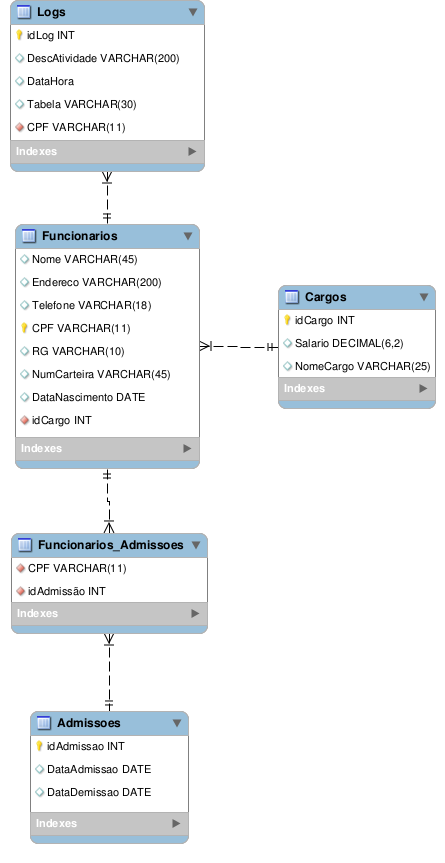
\includegraphics[width=9cm,keepaspectratio]{Imgs/ML_03}
         \caption{Modelo Lógico: Logs, Funcionários, Cargos, Funcionarios\_Admissoes e Admissoes.}
         \label{ml_03}
    \end{figure}
    
    \newpage
    
    A Figura \ref{ml_00} contém o modelo lógico completo.
    
    \begin{figure}[h]
         \centering
         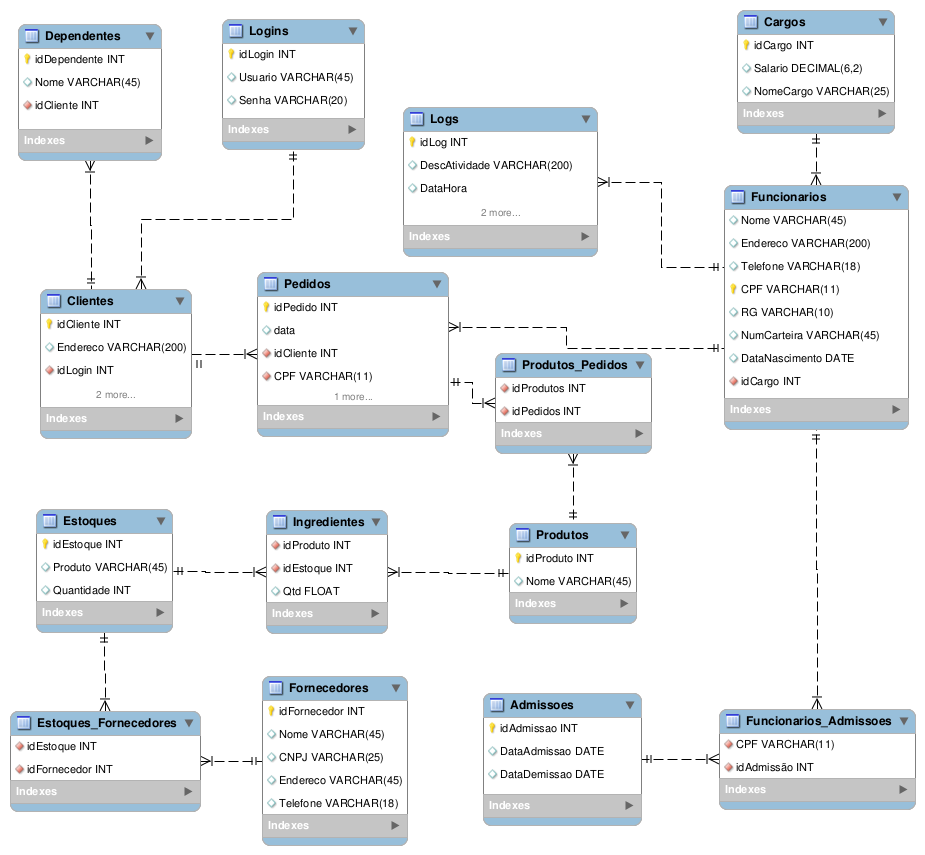
\includegraphics[width=20cm,keepaspectratio, angle=90]{Imgs/ML_00}
         \caption{Modelo Lógico completo.}
         \label{ml_00}
    \end{figure}

    
% ----------------------------------------------------------
% Implementação
% ----------------------------------------------------------
\chapter{Implementação}
    O banco de dados foi implementado utilizando o \textit{software SQL Server 2010}. Segue o código de execução para a criação das tabelas:
    
    \begin{lstlisting}
        USE master
        GO

        IF EXISTS (select name from sys.databases where name = 'Pizzaria')
                DROP DATABASE Pizzaria
        go

        CREATE DATABASE Pizzaria
        go

        USE Pizzaria
        go

        SET DATEFORMAT dmy
        go

        -- -----------------------------------------------------
        -- Table Pizzaria.Logins
        -- -----------------------------------------------------
        CREATE TABLE Logins (
          idLogin INT NOT NULL,
          Usuario VARCHAR(45) NULL,
          Senha VARCHAR(20) NULL,
          PRIMARY KEY (idLogin)
        )
        GO

        -- -----------------------------------------------------
        -- Table Pizzaria.Clientes
        -- -----------------------------------------------------
        CREATE TABLE Clientes (
          idCliente INT NOT NULL PRIMARY KEY,
          Nome VARCHAR (200) NOT NULL,
          Endereco VARCHAR(200) NULL,
          idLogin INT DEFAULT NULL,
          Telefone VARCHAR(18) NULL,
          CONSTRAINT fk_Clientes_Logins
            FOREIGN KEY (idLogin)
            REFERENCES Logins (idLogin)
            ON DELETE NO ACTION
            ON UPDATE NO ACTION
        )
        GO

        -- -----------------------------------------------------
        -- Table Pizzaria.Cargos
        -- -----------------------------------------------------
        CREATE TABLE Cargos (
          idCargo INT NOT NULL,
          Salario DECIMAL(6,2) NULL,
          NomeCargo VARCHAR(25) NULL,
          PRIMARY KEY (idCargo)
        )
        GO

        -- -----------------------------------------------------
        -- Table Pizzaria.Funcionarios
        -- -----------------------------------------------------
        CREATE TABLE Funcionarios (
          Nome VARCHAR(45) NULL,
          Endereco VARCHAR(200) NULL,
          Telefone VARCHAR(18) NULL,
          CPF VARCHAR(11) NOT NULL,
          RG VARCHAR(10) NULL,
          NumCarteira VARCHAR(45) NULL,
          DataNascimento DATE NULL,
          idCargo INT NOT NULL,
          PRIMARY KEY (CPF),
          CONSTRAINT fk_Funcionarios_Cargos
            FOREIGN KEY (idCargo)
            REFERENCES Cargos (idCargo)
            ON DELETE NO ACTION
            ON UPDATE NO ACTION
        )
        GO

        -- -----------------------------------------------------
        -- Table Pizzaria.Pedidos
        -- -----------------------------------------------------
        CREATE TABLE Pedidos (
          idPedido INT NOT NULL,
          data DATETIME NULL,
          idCliente INT NOT NULL,
          CPF VARCHAR(11) NOT NULL,
          Endereco VARCHAR(200) NULL,
          PRIMARY KEY (idPedido),
          CONSTRAINT fk_Pedidos_Clientes
            FOREIGN KEY (idCliente)
            REFERENCES Clientes (idCliente)
            ON DELETE NO ACTION
            ON UPDATE NO ACTION,
          CONSTRAINT fk_Pedidos_Funcionarios
            FOREIGN KEY (CPF)
            REFERENCES Funcionarios (CPF)
            ON DELETE NO ACTION
            ON UPDATE NO ACTION
        )
        GO

        -- -----------------------------------------------------
        -- Table Pizzaria.Dependentes
        -- -----------------------------------------------------
        CREATE TABLE Dependentes (
          idDependentes INT NOT NULL,
          Nome VARCHAR(45) NULL,
          idCliente INT NOT NULL,
          PRIMARY KEY (idDependentes),
          CONSTRAINT fk_Dependentes_Clientes
            FOREIGN KEY (idCliente)
            REFERENCES Clientes (idCliente)
            ON DELETE NO ACTION
            ON UPDATE NO ACTION
        )
        GO

        -- -----------------------------------------------------
        -- Table Pizzaria.Produtos
        -- -----------------------------------------------------
        CREATE TABLE Produtos (
          idProduto INT NOT NULL,
          Nome VARCHAR(45) NULL,
          PRIMARY KEY (idProduto)
        )
        GO

        -- -----------------------------------------------------
        -- Table Pizzaria.Estoques
        -- -----------------------------------------------------
        CREATE TABLE Estoques (
          idEstoque INT NOT NULL,
          Produto VARCHAR(45) NULL,
          Quantidade INT NULL,
          PRIMARY KEY (idEstoque)
        )
        GO


        -------------------------------------------------------
        -- Table Pizzaria.Ingredientes
        -------------------------------------------------------
        CREATE TABLE Ingredientes (
	        idProduto INT NOT NULL,
	        idEstoque INT NOT NULL,
	        Qtd FLOAT NOT NULL,
	        FOREIGN KEY (idProduto)
			        REFERENCES Produtos (idProduto)
			        ON DELETE NO ACTION
			        ON UPDATE NO ACTION,
	        FOREIGN KEY (idEstoque)
			        REFERENCES Estoques (idEstoque) 
			        ON DELETE NO ACTION
			        ON UPDATE NO ACTION
        )
        GO

        -- -----------------------------------------------------
        -- Table Pizzaria.Fornecedores
        -- -----------------------------------------------------
        CREATE TABLE Fornecedores (
          idFornecedor INT NOT NULL,
          Nome VARCHAR(45) NULL,
          CNPJ VARCHAR(25) NULL,
          Endereco VARCHAR(95) NULL,
          Telefone VARCHAR(18) NULL,
          PRIMARY KEY (idFornecedor)
        )
        GO

        -- -----------------------------------------------------
        -- Table Pizzaria.Estoques_Fornecedores
        -- -----------------------------------------------------
        CREATE TABLE Estoques_Fornecedores (
          idEstoque INT NOT NULL,
          idFornecedor INT NOT NULL,
          CONSTRAINT fk_Estoque_has_Fornecedor_Estoque
            FOREIGN KEY (idEstoque)
            REFERENCES Estoques (idEstoque)
            ON DELETE NO ACTION
            ON UPDATE NO ACTION,
          CONSTRAINT fk_Estoque_has_Fornecedor_Fornecedor
            FOREIGN KEY (idFornecedor)
            REFERENCES Fornecedores (idFornecedor)
            ON DELETE NO ACTION
            ON UPDATE NO ACTION
        )
        GO

        -- -----------------------------------------------------
        -- Table Pizzaria.Produtos_Pedidos
        -- -----------------------------------------------------
        CREATE TABLE Produtos_Pedidos (
          idProduto INT NOT NULL,
          idPedido INT NOT NULL,
          CONSTRAINT fk_Produtos_has_Pedidos_Produtos
            FOREIGN KEY (idProduto)
            REFERENCES Produtos (idProduto)
            ON DELETE NO ACTION
            ON UPDATE NO ACTION,
          CONSTRAINT fk_Produtos_has_Pedidos_Pedidos
            FOREIGN KEY (idPedido)
            REFERENCES Pedidos (idPedido)
            ON DELETE NO ACTION
            ON UPDATE NO ACTION
        )
        GO

        -- -----------------------------------------------------
        -- Table Pizzaria.Admissoes
        -- -----------------------------------------------------
        CREATE TABLE Admissoes (
          idAdmissao INT NOT NULL,
          DataAdmissao DATE NULL,
          DataDemissao DATE NULL,
          PRIMARY KEY (idAdmissao)
        )
        GO

        -- -----------------------------------------------------
        -- Table Pizzaria.Funcionarios_Admissoes
        -- -----------------------------------------------------
        CREATE TABLE Funcionarios_Admissoes (
          CPF VARCHAR(11) NOT NULL,
          idAdmissão INT NOT NULL,
          CONSTRAINT fk_Funcionarios_has_Admissão_Funcionarios
            FOREIGN KEY (CPF)
            REFERENCES Funcionarios (CPF)
            ON DELETE NO ACTION
            ON UPDATE NO ACTION,
          CONSTRAINT fk_Funcionarios_has_Admissão_Admissão
            FOREIGN KEY (idAdmissão)
            REFERENCES Admissoes (idAdmissao)
            ON DELETE NO ACTION
            ON UPDATE NO ACTION
        )
        GO

        -- -----------------------------------------------------
        -- Table Pizzaria.Logs
        -- -----------------------------------------------------
        CREATE TABLE Logs (
          idLog INT NOT NULL,
          DescAtividade VARCHAR(200) NULL,
          DataHora DATETIME NULL,
          CPF VARCHAR(11) NOT NULL,
          PRIMARY KEY (idLog),
          CONSTRAINT fk_Log_Funcionarios
            FOREIGN KEY (CPF)
            REFERENCES Funcionarios (CPF)
            ON DELETE NO ACTION
            ON UPDATE NO ACTION
        )
        GO
    \end{lstlisting}

% ----------------------------------------------------------
% Execução e Testes
% ----------------------------------------------------------
\chapter {Execução e Testes}
    As execuções e os testes foram feitos utilizando o \textit{software SQL Server Management Studio 2010}.
    
\section{Consultas}
    % Explicar
    A consulta a seguir foi realizada utilizando as tabelas Estoques e Fornecedores 
    e o resultado pode ser visualizado na figra \ref{select01}
    \begin{lstlisting}
-- -----------------------------------------------------
-- Lista alimentos e seus fornecedores
-- -----------------------------------------------------    
SELECT  Estoques.Produto as [Alimento], 
        Fornecedores.Nome as [Fornecedor] 
    FROM Estoques_Fornecedores
	    INNER JOIN Estoques ON 
	        Estoques.idEstoque = Estoques_Fornecedores.idEstoque 
	    INNER JOIN Fornecedores ON 
	        Fornecedores.idFornecedor = Estoques_Fornecedores.idFornecedor
	ORDER BY Fornecedores.Nome, Estoques.Produto
GO      
    \end{lstlisting}
    
    % Mostrar resultado
    \begin{figure}[h]
         \centering
         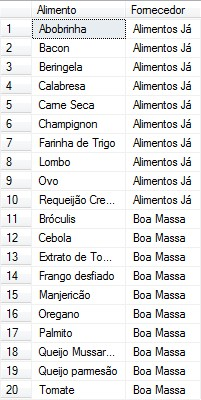
\includegraphics[width=6cm,keepaspectratio]{Imgs/Select_001}
         \caption{Resultado do select Lista alimentos e seus fornecedores}
         \label{select01}
    \end{figure}
    
    \newpage
    \newpage
    
    % Explicar
    A consulta a seguir foi realizada utilizando as tabelas Produtos e Estoques  
    e o resultado pode ser visualizado na figura \ref{select02}
    \begin{lstlisting}
-- -----------------------------------------------------
-- Lista os nomes dos produtos, seus ingredientes e a
-- quantidade em estoque
-- -----------------------------------------------------
SELECT  Produtos.Nome, 
        Estoques.Produto, 
        Estoques.Quantidade 
    FROM Ingredientes
	    INNER JOIN Produtos ON 
	        Produtos.idProduto = Ingredientes.idProduto 
    	INNER JOIN Estoques ON 
        	Estoques.idEstoque = Ingredientes.idEstoque 
	ORDER BY Produtos.Nome, Estoques.Produto
GO    
    
    \end{lstlisting}
    % Mostrar resultado
    \begin{figure}[h]
         \centering
         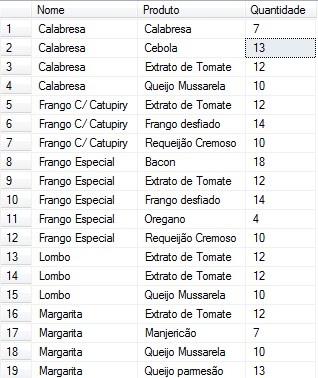
\includegraphics[width=10cm,keepaspectratio]{Imgs/Select_002}
         \caption{Resultado do select}
         \label{select02}
    \end{figure}

    \newpage
    
    % Explicar
    A consulta a seguir foi realizada utilizando as tabelas Logins e Clientes  
    e o resultado pode ser visualizado na figra \ref{select03}.
    \begin{lstlisting}
-- -----------------------------------------------------
-- Lista os clientes e os logins de quem o tiver.
-- -----------------------------------------------------
CREATE VIEW ClientesComLogin
AS
	SELECT  Logins.Usuario, 
    	Clientes.idCliente FROM Logins
	    	RIGHT JOIN Clientes ON 
    	Logins.idLogin = Clientes.idLogin 
GO
    
    \end{lstlisting}
    % Mostrar resultado
    \begin{figure}[h]
         \centering
         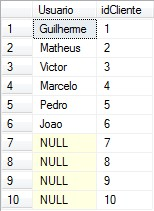
\includegraphics[width=5cm,keepaspectratio]{Imgs/Select_003}
         \caption{Resultado do select lista os clientes e os logins de quem o tiver.}
         \label{select03}
    \end{figure}
    
    \newpage
    
    %Explicar
    A consulta a seguir foi realizada utilizando as tabelas Produtos e Pedidos 
    e o resultado pode ser visualizado na figra \ref{select04}.
    \begin{lstlisting}
-- -----------------------------------------------------
-- Lista produtos pedidos
-- -----------------------------------------------------
CREATE VIEW PedidosRealizados
AS 
	SELECT  Produtos.Nome AS [Produto], 
	        Pedidos.idCliente 
        FROM Produtos_Pedidos
		    INNER JOIN Produtos ON 
		        Produtos.idProduto = Produtos_Pedidos.idProduto 
		    INNER JOIN Pedidos ON 
		        Pedidos.idPedido = Produtos_Pedidos.idPedido 
GO    
    
    \end{lstlisting}
    % Mostrar resultado
    \begin{figure}[h]
         \centering
         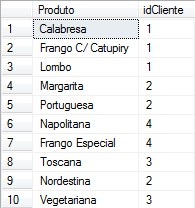
\includegraphics[width=10cm,keepaspectratio]{Imgs/Select_004}
         \caption{Resultado do select lista produtos pedidos.}
         \label{select04}
    \end{figure}

    \newpage

    % Explica
    A consulta a seguir foi realizada utilizando as views ClientesComLogin e PedidosRealizados
    e o resultado pode ser visualizado na figra \ref{select05}.
    \begin{lstlisting}
-- -----------------------------------------------------
-- Lista dos clientes que fizeram pedidos.
-- -----------------------------------------------------
CREATE VIEW ClientesQueFizeramPedidos
AS
SELECT	ClientesComLogin.Usuario,
		PedidosRealizados.Produto
		 FROM PedidosRealizados
	INNER JOIN ClientesComLogin ON 
	    ClientesComLogin.idCliente = PedidosRealizados.idCliente
GO


SELECT  ClientesQueFizeramPedidos.Usuario, 
        COUNT(*) AS [Quantidade de Pedidos] 
    FROM ClientesQueFizeramPedidos 
	    GROUP BY ClientesQueFizeramPedidos.Usuario
    
    \end{lstlisting}
    % Mostrar resultado
    \begin{figure}[h]
         \centering
         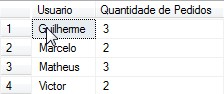
\includegraphics[width=10cm,keepaspectratio]{Imgs/Select_005}
         \caption{Resultado do select lista dos clientes que fizeram pedidos.}
         \label{select05}
    \end{figure}
    
    \newpage
    
    % Explicar
    A consulta a seguir foi realizada utilizando a view ClientesComLogin e a tabela Dependentes 
    e o resultado pode ser visualizado na figra \ref{select06}.    
    \begin{lstlisting}
-- -----------------------------------------------------
-- Clientes e seus dependentes
-- -----------------------------------------------------
SELECT  ClientesComLogin.Usuario, 
        Dependentes.Nome [Nome do dependente] 
    FROM Dependentes
	    INNER JOIN ClientesComLogin ON 
	        ClientesComLogin.idCliente = Dependentes.idCliente
    
    \end{lstlisting}
    % Mostrar resultado
    \begin{figure}[h]
         \centering
         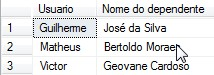
\includegraphics[width=10cm,keepaspectratio]{Imgs/Select_006}
         \caption{Resultado do select clientes e seus dependentes} 
         \label{select06}
    \end{figure}

    \newpage
    
    % Explicar
    A consulta a seguir foi realizada utilizando as tabelas Funcionários e Cargos
    e o resultado pode ser visualizado na figra \ref{select07}. 
    \begin{lstlisting}
-- -----------------------------------------------------
-- Funcionários e Cargos
-- -----------------------------------------------------
SELECT  Funcionarios.Nome, 
        Funcionarios.CPF, 
        Cargos.NomeCargo, 
        Cargos.Salario 
    FROM Funcionarios
	    INNER JOIN Cargos ON
	        Cargos.idCargo = Funcionarios.idCargo
	ORDER BY Cargos.NomeCargo, Funcionarios.Nome
GO  
    \end{lstlisting}
    % Mostrar resultado
    \begin{figure}[h]
         \centering
         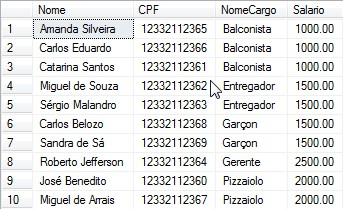
\includegraphics[width=10cm,keepaspectratio]{Imgs/Select_007}
         \caption{Resultado do select Funcionários e Cargos}
         \label{select07}
    \end{figure}    
    
    \newpage
    
    % Explicar
    A consulta a seguir foi realizada utilizando as tabelas Funcionários e Cargos
    e o resultado pode ser visualizado na figra \ref{select08}. 
    \begin{lstlisting}
    
-- -----------------------------------------------------
-- Funcionários, cargos e suas admissões
-- -----------------------------------------------------
SELECT  Funcionarios.Nome, 
        Admissoes.DataAdmissao, 
        Cargos.NomeCargo, 
        Cargos.Salario 
    FROM Funcionarios_Admissoes
	    INNER JOIN Funcionarios ON 
	        Funcionarios.CPF = Funcionarios_Admissoes.CPF 
	    INNER JOIN Admissoes 
	        ON Admissoes.idAdmissao = Funcionarios_Admissoes.idAdmissão 
	    INNER JOIN Cargos 
	        ON Cargos.idCargo = Funcionarios.idCargo
GO

    
    \end{lstlisting}
    % Mostrar resultado
    \begin{figure}[h]
         \centering
         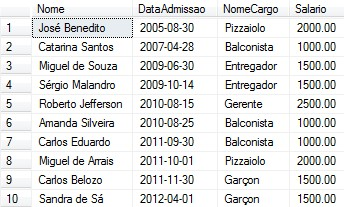
\includegraphics[width=10cm,keepaspectratio]{Imgs/Select_008}
         \caption{Resultado do select funcionários, cargos e suas admissões}
         \label{select08}
    \end{figure}
    
    \newpage
       
\section{Procedimentos armazenados}

    % Explicar
    Procedimento armazenado para cálculo do aniversários de cada funcionário na empresa.
    \begin{lstlisting}
CREATE PROCEDURE usp_idadeFuncionarios
AS
	SELECT  Nome, 
	        DATEDIFF(YEAR, DataNascimento, GETDATE()) - CASE 
					WHEN GETDATE() < DATEADD(YEAR, 
					    DATEDIFF(YEAR,DataNascimento, 
                                 GETDATE()), 
				                 DataNascimento)
						THEN 1
						ELSE 0
					END AS 'Idade',  
					        CONVERT(VARCHAR(10), 
					        DataNascimento, 103) As 'Data de Nascimento'
    	FROM Funcionarios
GO

EXEC usp_idadeFuncionarios
GO
    \end{lstlisting}
    
    Depois de executado, o reultado obtido pode ser visualizado na Figura \ref{usp_001}.
    
    % Mostrar resultado
    \begin{figure}[h]
         \centering
         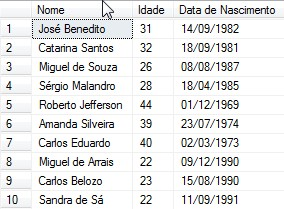
\includegraphics[width=10cm,keepaspectratio]{Imgs/USP_001}
         \caption{Procedimento Armazenado para calcular idade.}
         \label{usp_001}
    \end{figure}
    
    \newpage
    
    % Explicar
    \begin{lstlisting}
CREATE PROCEDURE usp_pedidosRealizados
	@nome VARCHAR(45)
AS
	SELECT  F.Nome, 
	        C.NomeCargo as 'Cargo', 
	        Prod.Nome, 
	        CONVERT(VARCHAR(10),P.data, 103) As 'Data do Pedido'  
        FROM Funcionarios F
            INNER JOIN Cargos C ON 
                C.idCargo = F.idCargo
            INNER JOIN Pedidos P ON 
                P.CPF = F.CPF
            INNER JOIN Produtos_Pedidos PP ON 
                PP.idPedido = P.idPedido
            INNER JOIN Produtos Prod ON 
                Prod.idProduto = PP.idProduto
        WHERE F.Nome = @nome     
GO
    \end{lstlisting}
    
    % Mostrar resultado
    Depois de executado, o reultado obtido pode ser visualizado na Figura \ref{usp_002}.
    \begin{figure}[h]
         \centering
         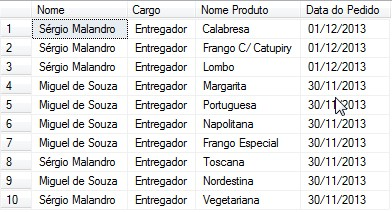
\includegraphics[width=10cm,keepaspectratio]{Imgs/USP_002}
         \caption{Resultado do procedimento armazenado que retorna os pedidos realizados.}
         \label{usp_002}
    \end{figure}
    
    \newpage
    
    % Explicar
    \begin{lstlisting}
CREATE PROCEDURE usp_pedidosRealizadosCliente
	@nome VARCHAR(45)
AS
	SELECT  Cli.Nome, 
	        Prod.Nome, 
	        CONVERT(VARCHAR(10), 
	        P.data, 103) As 'Data do Pedido'  
    FROM Clientes Cli
        INNER JOIN Pedidos P ON 
            P.idCliente = Cli.idCliente
        INNER JOIN Produtos_Pedidos PP 
            ON PP.idPedido = P.idPedido
        INNER JOIN Produtos Prod 
            ON Prod.idProduto = PP.idProduto
        WHERE Cli.Nome = @nome     
GO
    \end{lstlisting}
    
    Depois de executado, o reultado obtido pode ser visualizado na Figura \ref{usp_003p1} e 
    também na Figura \ref{usp_003p2}.
    % Mostrar resultado
    \begin{figure}[h]
         \centering
         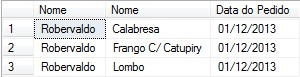
\includegraphics[width=10cm,keepaspectratio]{Imgs/USP_003p1}
         \caption{Procedimento Armazenado que retorna os pedidos de um determinado cliente via parâmetro do nome.}
         \label{usp_003p1}
    \end{figure}
    
    \begin{figure}[h]
         \centering
         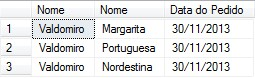
\includegraphics[width=10cm,keepaspectratio]{Imgs/USP_003p2}
         \caption{Procedimento Armazenado que retorna os pedidos de um determinado cliente via parâmetro do nome.}
         \label{ups_003p2}
    \end{figure}

% ---
% Finaliza a parte no bookmark do PDF
% para que se inicie o bookmark na raiz
% e adiciona espaço de parte no Sumário
% ---
%\phantompart

% ---
% Conclusão
% ---
\chapter*[Considerações]{Considerações Finais}
\addcontentsline{toc}{chapter}{Considerações Finais}

Apesar de parecer simples, criar um banco de dados para uma pizzaria mostrou-se 
uma tarefa cheia de detalhes a se pensar. Ao ser implementado, tornou-se 
funcional, sendo possível utilizá-lo em um ambiente real.

% ----------------------------------------------------------
% ELEMENTOS PÓS-TEXTUAIS
% ----------------------------------------------------------
\postextual

% ----------------------------------------------------------
% Referências bibliográficas
% ----------------------------------------------------------
% \bibliography{abntex2-modelo-references}
\bibliography{ref}

% ----------------------------------------------------------
% Glossário
% ----------------------------------------------------------
%
% Consulte o manual da classe abntex2 para orientações sobre o glossário.
%
%\glossary

% ----------------------------------------------------------
% Apêndices
% ----------------------------------------------------------

% ---
% Inicia os apêndices
% ---
% \begin{apendicesenv}

% % Imprime uma página indicando o início dos apêndices
% \partapendices

% % ----------------------------------------------------------
% \chapter{Quisque libero justo}
% % ----------------------------------------------------------

% \lipsum[50]

% % ----------------------------------------------------------
% \chapter{Nullam elementum urna vel imperdiet sodales elit ipsum pharetra ligula
% ac pretium ante justo a nulla curabitur tristique arcu eu metus}
% % ----------------------------------------------------------
% \lipsum[55-57]

% \end{apendicesenv}
% ---


% ----------------------------------------------------------
% Anexos
% ----------------------------------------------------------

% ---
% Inicia os anexos
% ---
\begin{anexosenv}

% % Imprime uma página indicando o início dos anexos
\partanexos

% % ---
\chapter{Dados inseridos para teste}
% % ---
\lipsum[30]

%\lstinputlisting{../Sql/Inserts.sql}

\end{anexosenv}

%---------------------------------------------------------------------
% INDICE REMISSIVO
%---------------------------------------------------------------------

%\phantompart
\printindex

\end{document}
